\chapter{Information Systems Models and Frameworks} \label{chap:inf-sys}

\section*{}

%Neste capítulo é descrito o estado da arte e são
%apresentados trabalhos relacionados para mostrar o que existe no
%mesmo domínio e quais os problemas em aberto.
%Deve deixar claro que existe uma oportunidade de desenvolvimento que
%cobre alguma falha concreta .
%
%O capítulo deve também efectuar uma revisão tecnológica às principais
%ferramentas utilizáveis no âmbito do projecto, justificando futuras
%escolhas.


%TODO secção inicial sobre information systems
%\section{Health Information Systems}
%
%\subsection{Information Systems}
%
%%Falar sobre os sistemas de informação de forma genérica
%
%\subsection{Portugal overview}\label{sec:dialecto}
%

In this chapter we present a general study about how is it possible to build ultra-large systems. The Information Systems (IS) are a kind of large dimension systems. The development methods used to implement these systems are an important source of experiences and techniques relevant to this dissertation. The first section describes some Enterprise Architecture Frameworks and in the second one we introduce three Architectural Models.


\section{Enterprise Architecture Frameworks} \label{sec:ea-frams}
The concept of Enterprise Architecture appeared more than 20 years ago. At that time, the systems complexity was growing with an exponential velocity. However, most of the times, those systems were not able to fulfil the business needs and the problem was not lack of technology or knowledge but difficulties in understanding the business from those who were developing it. Thus, the software development was facing two problems at a time: in one hand, the systems were becoming huge and hugely complex; on the other hand, the systems were developed with few concerns about business orientation~\citep{Sessions2007}.

Despite of being a problem with a considerable age and very studied also, it did not stop growing and there is not a quite clear solution. A lot of enterprise architecture models appeared and disappeared over the years. However, it is estimated that around 90\% of the market is dominated by this four methodologies~\citep{Sessions2007}:

\begin{itemize}
\item The Zachman Framework;
\item The Open Group Architecture Framework (TOGAF);
\item The Federal Enterprise Architecture Framework (FEAF);
\item The Gartner Methodology. %TODO rever ou tirar-- atençao à referncia
\end{itemize}

In the next subsections, we will slightly describe each one of them, trying to understand which the advantages and weak points of each one. 











\subsection{The Zachman Framework} \label{sec:zachman-fw}

The Zachman Framework~\citep{Zachman1987} aims to guarantee that all stakeholders' perspectives are being taken into account when developing a complex software system. In general terms, it is important to understand if all the artefacts are sufficiently focused and if the existing artefacts clarify all the players, from the business owner till the database designer, keeping all the visions aligned.

In the original article and in order to explain his methodology, John Zachman uses an analogy between building an information system and construct a building. Thus, when constructing a building, the architect starts with understanding the general requirements as how many divisions it is supposed to have and the general purpose of the building, usually by using bubble charts. In a second phase, the architect's drawings aims to represent the links between each room of the building and also its general structure. Finally, the architect presents the plans and they must represent and reflect the customer requirements and expectations. These plans already include several details about electrical system, masonry, wood structure, etc. After plans arrive the contractor, they suffer some adjustments either because of costs/price or because another kind of constructing limitations.

In general, we can say that there are three fundamental architectural representations, one for each player in this process: the owner, the designer and the builder. Through all this process, the project will be documented in many perspectives. The architect starts listening to the customer and building his own perspective of the project that is sent to the builder, which in turn builds another view that allows himself to clarify some aspects. Despite of all these documents refer and describe the same project, each one of them has different purposes. Each one of them is unique and independent, describes one area, one perspective, not being possible from one of those to conclude about the others.

Originally, the proposal of Zachman was based on a policy of three questions: What?, How? and Where?, used to describe the product. However, the model has evolved and now it is based in three more questions: Who?, When? and Why?.

\addtocounter{footnote}{1}
\begin{figure}[t]
\centering
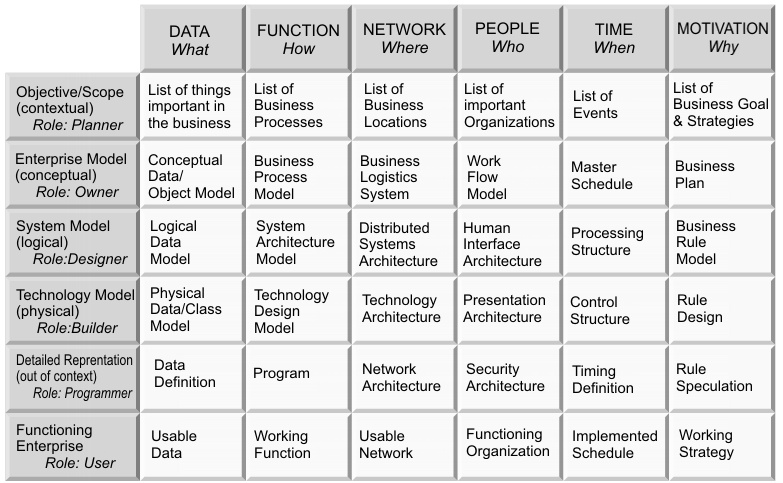
\includegraphics[width=1.0\textwidth]{zachman-framework}
\caption[Zachman Framework classification model]%
			{Zachman Framework classification model$^{\decimal{footnote}}$}
\label{fig:zachman-architecture}
\end{figure}

Just as it is possible to see in Figure~\ref{fig:zachman-architecture}, Zachman claims a classification of the existing artefacts from multiple points of view, identifying:
\begin{itemize}
\item \textbf{Material description} --- the data model of the system: ``entity - relationship - entity''; 
\item \textbf{Functional description} --- the process model of the system: ``input - process - output'';
\item \textbf{Location description} --- the network model of the system: ``node - line - node'';
\item \textbf{People description} --- the organization units and roles within the system: ``organization - reporting - organization'';
\item \textbf{Time description} --- the events of the system: ``event - cycle - event'';
\item \textbf{Motivation description} --- the high level organization goals of the system: ``node - line - node''.
\end{itemize}

\footnotetext[\value{footnote}]{Source: \url{http://upload.wikimedia.org/wikipedia/commons/d/da/Zachman_Framework_Detailed.jpg}}

%A forma como os três intervenientes vê cada entidade do sistema retrata-se também no artigo. De facto, quando o cliente se refere a um empregado está a referir-se à pessoa enquanto que o constructor está a pensar num registo no sistema, dessa entidade.

Over the years, this model started to be considered more like a taxonomy model, helping to frame all the artefacts and state their value and meaning to the multiple stakeholders~\citep{Sessions2007}.






\subsection{The Open Group Architecture Framework} \label{sec:togaf}

First developed in 1995, The Open Group Architecture Framework was based on the US Department of Defense Technical Architecture Framework for Information Management (TAFIM). From this sound foundation, The Open Group Architecture Forum has developed successive versions of TOGAF at regular intervals and published them on The Open Group public web site~\citep{Josey2011}.

TOGAF might be seen as a process for building an Enterprise Architecture. This framework states this building process as a continuous process of building multiple architectures from highly generic to highly specific ones, until reaching the organizational architecture level~\citep{Sessions2007}.

This framework splits the EA in four categories: 
\begin{itemize}
\item \textbf{Business Architecture} --- describes processes used by business to meet own goals;
\item \textbf{Application Architecture} --- describes how to build applications from the framework and how to interact with the other ones;
\item \textbf{Data Architecture} --- describes how the information is stored, organized and accessed;
\item \textbf{Technical Architecture} --- describes the hardware and software supporting the applications and their interactions.
\end{itemize}

One of the most important concepts of this framework is the Architecture Development Method (ADM), which stands as a reliable and proven approach for building enterprise architecture descriptions, keeping the progress close to the business specific needs. Actually, it provides an overall process template for architecture development activity and a narrative of each architecture phase, describing each one in terms of objectives, approach, inputs, steps and outputs to the architects~\citep{Leist2006}.

The TOGAF ADM also provides several guidelines and techniques:
\begin{itemize}
\item \textbf{Architecture Content Framework} --- detailed model for architectural work products, including deliverables and artefacts;
\item \textbf{Enterprise Continuum} --- a model for structuring a virtual repository and classify architecture and solution artefacts, tracking how the artefacts evolve and how they can be re-used;
\item \textbf{TOGAF Reference Models} --- two reference models: Technical Reference Model (TRM) and Integrated Information Infrastructure Model (III-RM);
\item \textbf{Architecture Capability Framework} --- a set of templates, guidelines, resources that aim to help the architect establishing some practices within an organization.
\end{itemize}

In overall terms, TOGAF ADM recommends an iterative process for architecture development, not being prescriptive on breadth of coverage, level of details or time horizons. The architect determines those details to fit one specific project. One of the most important characteristics of TOGAF ADM is that, despite of having well-defined phases, it enough flexible to be adapted to the organization and to let architects build the best approach to implement TOGAF~\citep{Tang2004}.









\subsection{Federal Enterprise Architecture Framework} \label{sec:feaf}

The Federal Enterprise Architecture Framework appeared with the objective of serving as a platform for sharing processes, information and documentation among the U.S. Federal Agencies and other government agencies. This framework gathers two main characteristics of the two previous: in on hand, it defines a taxonomy -- similar to the Zachman Framework (Section \ref{sec:zachman-fw}) -- for artefacts classification; on the other hand, it suggests a process for building and implementing the architecture like TOGAF (Section \ref{sec:togaf}) does. 

The FEAF partitions a given `platform' into business, data, applications and technologies architectures, aiming to take those into account when applying the process of implementing the new architecture. Furthermore, the framework is organized in four levels~\citep{Tang2004}:
\begin{itemize}
\item Level I --- the highest level which deals with the architecture drivers or external stimulus fetching the strategic direction of the architecture. It facilitates the transformation from the original architecture to the new one by applying architecture standards and managing the process;
\item Level II --- an analyses of the business goals, direction, principles, strategies and priorities;
\item Level III --- expression of architecture in more detailed view by using business data, applications and technology views to model it;
\item Level IV --- representation of Data Architecture, Application Architecture and Technology Architecture using a combination of Zachman Framework and Spewak's Enterprise Architecture Planning methods.
\end{itemize}

% Success measurement
FEAF also suggests a measurement process, being able to evaluate the maturity the inner organizations are adopting and implementing the enterprise architecture. This evaluation classifies the agencies measuring three essential attributes: 
\begin{itemize}
\item Architectural completion --- the maturity of the architecture itself;
\item Architectural use --- how is the architecture being used to improve efficiency of decision-making;
\item Architectural results --- the benefits brought by the use of the architecture.
\end{itemize}

Based on the analysis of this three attributes, the agencies are then rated in one of three categories: green, yellow and red. 

%Antes de abordar as diferentes recomendações da FEA importa referir alguns conceitos fundamentais: 
%- segmentos: segmentos de missão central (ex: educação para o Min. Educação) e segmentos de serviços de negócio (ex: gestão financeira)
%- serviços empresariais (ex: gestão de segurança)

%Modelos de referência do FEA 
%- modelo de referência de negócio
%- modelo de referência de componentes
%- modelo técnico de referência
%- modelo de referência de dados- modelo de referência de performance

%Processo do FEA
%1) análise arquitectural
%2) definição da arquitectura
%3) estratégia de financiamento e investimento
%4) gestão do planeamento e execução do projecto




%\subsection{Gartner Enterprise Architecture}
%
%Gartner não pode ser descrito nem como um processo taxonómico, nem como um processo, muito menos como uma metodologia completa. Em vez disso, pode definir-se como uma prática. É uma práctica para arquitecturas empresariais realizada por uma empresa de consultadoria, a Gartner.
%  
%Esta prática não se baseia no que a empresa é, mas naquilo que quer ser, nos objectivos que pretende atingir. Acredita-se que o fundamental está em formar uma equipa constituida por pessoas do negócio, especialistas em informação e os responsáveis de implementação. O essencial para por criar neste grupo de pessoas uma visão comum para a empresa.





\section{Architectural Styles} \label{sec:arch-styles}

An Architectural Style is a particular pattern that organizes components and connectors in a particularly form, providing a well-known reliable solution when facing a specific kind of problem~\citep{Kazman}. Each architectural style principle influences some quality attributes in a positive and some other in a negative way. Zheng Qin \textit{et al} define it as ``a solution to solve a certain class of problems which have common quality attributes requirements'', stating also that ``there is no architecture style that is proper for all systems, because every system have different quality attributes requirements''~\citep{Qin2008}. Kim and Garlan advocate~\citep{Kim2010} that these concepts bring a number of significant benefits as they promote design reuse.

\subsection{The Metropolis Model} \label{sec:metro-model}

Over the last years, two important trends are changing business and society: in one hand, the growing use of shared knowledge to create high-value services and projects; on the other hand, the growing preponderance of services. The businesses are evolving from a product-oriented perspective to a relation-oriented one. This change of paradigm brought the client to the middle of the business, helping to create value. The greatest examples of this new philosophy are the systems based in communities as Wikipedia or Facebook, that are able to generate profit and value directly from its users.

The Metropolis Model~\citep{Kazman2009} appears as an attempt of describing really huge complex systems built from two basilar concepts: Open-source Software (OSS) and Community-Based Service Systems (CBSS). Despite the growing importance of OSS and CBSS, there will always be some systems that cannot be developed by crowds, either because of the business criticality or for demanding unquestionable security guarantees. The Metropolis Model does not really apply to those systems.

We will start with an explanation of the ``crowdsourced systems'' and then briefly describe the principles of the Metropolis Model, always following the original article wrote by Rick Kazman and Hong-Mei Chen~\citep{Kazman2009}.

\subsubsection{Crowdsourced Systems}

The Metropolis Model identify its target as the ``crowdsourced systems''. This concept includes the kind of systems with some special characteristics:
\begin{itemize}
\item open teams --- meaning that the assumption of having a closed and dedicated team of programmers should be abandoned;
\item ``mashability'' --- as the capacity of composing and integrating different systems and functionalities since that
the consumption of software by one person or project does not make it less available for consumption by another;
\item conflicting, not knowable requirements --- the requirements emerge from the contributors and the users, making them highly unpredictable and often being in conflict between each other;
\item continuous evolution --- as a consequence of constant changing requirements and distributed resources, these type of systems are never finished nor stable, introducing the ``perpetual beta'' concept. The development of the project is done through multiple iterations empowering the users with the responsibility of testing and assuring its quality;
\item focus on operations --- the availability of its operations are, most of the times, as critical as their utility and, in that sense, it is not accepted any kind of system downtime (Amazon, eBay or Google are good examples);
\item sufficient correctness --- the notion of `perpetual beta' expresses the idea of acceptance some incompleteness in software (e.g. Wikipedia);
\item unstable resources --- one of the most interesting facts is that, despite of the volatility of people, information and other resources that individually would be useless, when massive congregated are able to create reliable, stable and impressive computational powered systems;
\item emergent behaviours --- frequently, there are behaviours and tendencies that emerge from the system that are completely unexpected. In these systems, unlike the traditional ones, the crowds take the rudder and bring to the system unpredicted kinds of utilization or interaction.
\end{itemize}

\subsubsection{The principles}

The Metropolis Model presents a new unified vision between the CBSS and the OSS, focusing deliberately in the crowd value generation. This model suggests the creation of two levels: the kernel services and the periphery services. It states that the application's kernel may be developed using traditional methods.

The Metropolis Model is supported by the application of some principles:
\begin{itemize}
\item \textbf{Crowd engagement and egalitarian management of open teams} --- the management must focus the people and the crowds, engaging the users for value co-creation. The engagement is not just a system-level issue, but a question of business strategy. These kind of system resort to crowd-sourcing chasing ``potential for cost reduction, increased innovation, and quicker development time for delivering products and services that meet customer needs'' as the authors explain;
\item \textbf{Bifurcated requirements} --- the requirements must be distinguished into kernel or periphery ones. The kernel should ``deliver little or no end-user value'' (e.g. Linux kernel, Wikipedia wiki or Facebook application platform). On the other hand, from the periphery appears most of the end-user value, as it happens with Wikipedia articles or Facebook applications; 
\item \textbf{Bifurcated architecture} --- the architecture of these systems are composed by the kernel infrastructure and the peripheral services. Since the kernel must be designed and implemented to be stable and promote the integration of several components, it must not emerge from the use of the system;
\item \textbf{Fragmented implementation} --- the crowd-sourced philosophy must be applied only to the peripheral services. The kernel implementation shall be done by an ``close-knit, highly motivated, coordinated team'', ensuring its high quality.
\item \textbf{Distributed testing} --- while the kernel must be highly reliable and constantly tested, in the peripheral services it is only necessary the sufficient correctness;
\item \textbf{Distributed delivery/maintenance} --- at the kernel level, it is important to preserve backwards compatibility when deploying a new version. At periphery the release mechanisms are uncoordinated and form a constant stream;
\item \textbf{Ubiquitous operations} --- these systems are ``always on'' even when they are being upgraded. Also, they should monitor self state and create control mechanisms not allowing peripheral problems to affect the system's core. 
\end{itemize}


\subsection{Service-oriented Architectures} \label{sec:soa}


A Service-oriented Architecture (SOA) is ``an architectural style that emphasizes implementation of components as modular services that can be discovered and used by clients'' and that ``emphasis on loose coupling between interacting services'' \citep{Srinivasan2005}. However, as Thomas Erl stated~\citep{Erl2005} there is no single definition of SOA. Instead, there are many opinions about what constitutes service-orientation. Erl advocates that the service-orientation paradigm has it ``roots in a software engineering theory known as separation of concerns''. Obviously, this concept has been applied in many contexts and to many platforms, from object-oriented programming till component-based programming approaches.

The service-orientation paradigm has no official principles. Although, there are ``a common set of principles most associated with service-orientation''~\citep{Erl2005}:
\begin{itemize}
\item \textbf{Services are reusable} --- the services are designed to promote and support their reuse, regardless of whether immediate reuse opportunities exist;
\item \textbf{Services share a formal contract} --- in order to be possible to share, there is a necessity for stablish the terms of information exchange;
\item \textbf{Services are loosely coupled} --- services must be designed to avoid dependency outside itself;
\item \textbf{Services abstract underlying logic} --- the only part visible to the outside is the interface and the requirements that need to be met to obtain the service, and that are clarified in the contract's description;
\item \textbf{Services are ``composable''} --- services might be aggregated with the finality of creating larger services, obtaining different abstraction levels and promoting re-utilization;
\item \textbf{Services are autonomous} --- the service is governed within an explicit boundary not being dependent to perform its operations;
\item \textbf{Services are stateless} --- services should not be required to manage state information as that might preclude their ability to stay independent and not coupled. The concerning about maximizing the statelessness must be central.
\end{itemize}

To conclude, as Srinivasan and Treadwell advocates~\citep{Srinivasan2005} ``service-orientation reinforces general software architecture principles such as encapsulation, modularization and separation of the interfaces from their implementations''.




\subsection{Event-driven Architectures}\label{sec:eda}

The Event-driven Architectures (EDA) are based in the event concept. An event~\citep{Michelson2006} is a notable thing that starts inside or outside the system and may consist in a problem, an opportunity and so forth. The event meaning should be defined in the business context. In an EDA, when an event is triggered it is immediately disseminated to every interested parties~\citep{Qin2008}. Then, these parties evaluate the event and might either call a service, trigger another component or simply take no action.

This architectural pattern promote loosely coupled and highly distributed systems. In fact, the creator of the event only has the task of dispatching it. From that point on, the creator loses track of the event, not knowing nothing about the post processing or even who are the interested parties. Usually, these architectures are defined by three main concepts:
\begin{itemize}
\item event trigger --- triggers the event sending it to the event collector;
\item event collector --- redirects the received events to the interested parties;
\item interested party --- receives the event information and proceeds in accordance, calling another component or service;
\end{itemize}

This basic structure might be scaled, allowing to organize and build much complex systems.

To conclude, it is important to say that these architectures are advisable to be used for asynchronous flows of work and information. Also, these architectural styles easily combine for creating robuster solutions~\citep{Marechaux2006,Laliwala2008}.

